In Fig.~\ref{fig:ratio2d_LO}, ratios of double-differential cross sections in the variables  $m_{\Pj\Pj}$ and $|\Delta y_{\Pj\Pj}|$ are shown.\footnote{In Fig.~\ref{fig:ratio2d_LO}, the level of the accuracy of the predictions in each bin is around a per mille.}
Two plots are displayed: the ratios of the $|t|^2 + |u|^2$ and $|s|^2 + |t|^2 + |u|^2$ approximations over the full calculation.
In the first case, the approximation is good within $\pm10\%$ over the whole range apart in the low invariant-mass region at both low and large rapidity difference.
The low rapidity-difference region possesses remnants of the tri-bosons contributions that have a di-jet invariant mass around the $\PW$-boson mass.
It is therefore expected that the $|t|^2 + |u|^2$ approximation fails in this region.
The second plot, where the $|s|^2 + |t|^2 + |u|^2$ approximation is considered, displays a better behaviour in the previously mentioned region.
The full calculation is approximated at the level of $\pm5\%$ apart in the region where $|\Delta y_{\Pj\Pj}| < 2$.

\begin{figure*}[hbt]
\centering
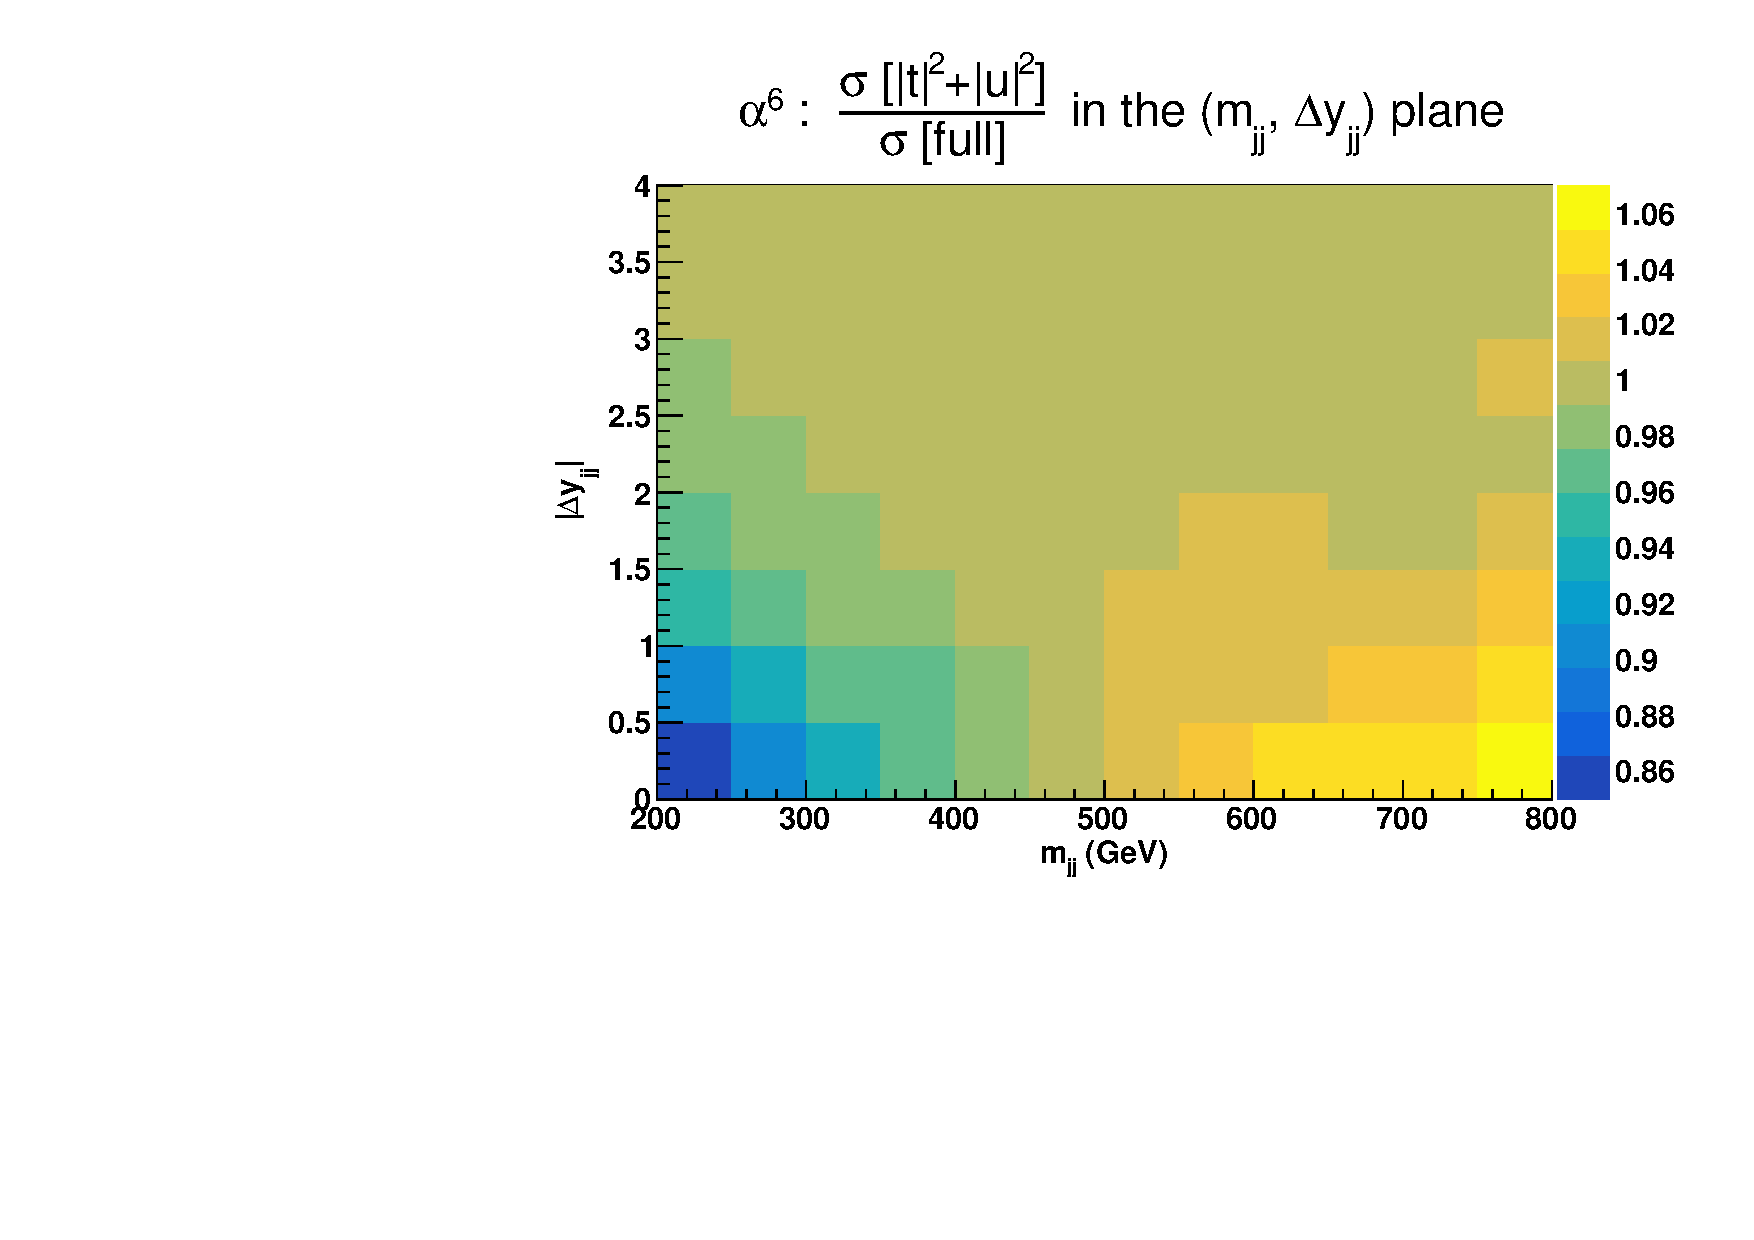
\includegraphics[scale=0.395]{figures/scanfigures/ratio_tu.pdf}
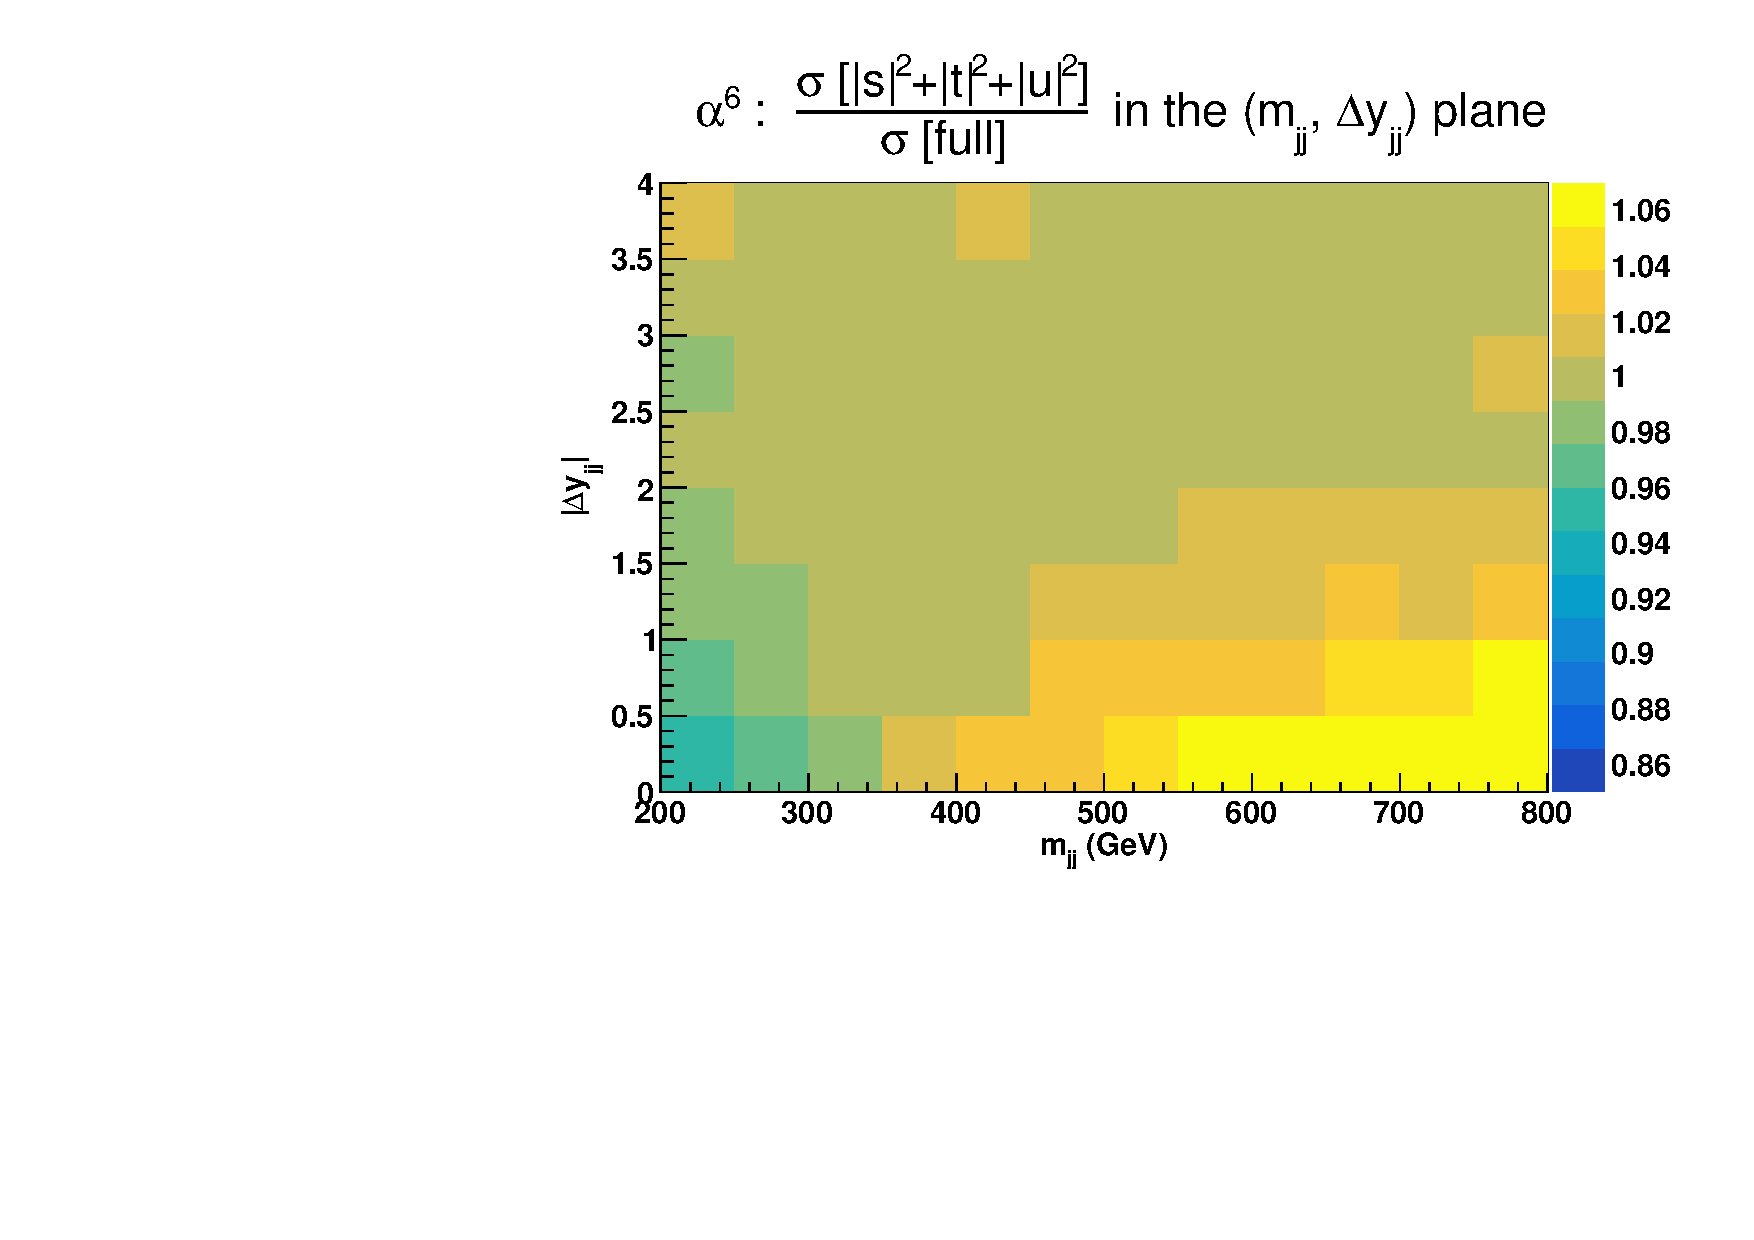
\includegraphics[scale=0.395]{figures/scanfigures/ratio_stu.pdf}
\caption{Ratios of double-differential distributions in the variables $m_{\Pj\Pj}$ and $|\Delta y_{\Pj\Pj}|$ at LO \emph{i.e.}\ order $\mathcal{O}(\alpha^6)$.
Ratio of approximated squared amplitudes over the full matrix element.
The approximated squared amplitudes are computed as $|\mathcal{A}|^2 \sim |t|^2 + |u|^2$ (left) and $|\mathcal{A}|^2 \sim |s|^2 + |t|^2 + |u|^2$ (right).
The cuts applied are the ones of Sec.~\ref{subsec:inputpar} and no cuts on $m_{\Pj\Pj}$ and $|\Delta y_{\Pj\Pj}|$ are applied.} 
\label{fig:ratio2d_LO}
\end{figure*}
% As explained previously, the low di-jet invariant mass and low jet rapidity separation regions are dominated by tri-boson production.

% Therefore, the \emph{inclusive} study at NLO is only performed in the region 
% %
% \begin{equation}
% \label{eq:inclusive}
% 	m_{jj} > 200\GeV\, \qquad {\rm and} \qquad |\Delta y_{jj}| > 2 .
% \end{equation}
% %
% Hence, the differences arising at NLO in this fiducial region originate solely from NLO effects.

% As explained previously, the low di-jet invariant mass are dominated by tri-boson production.
% Therefore, a comparison of the various approximations in an \emph{inclusive} phase-space volume should exclude the region where tri-boson contributions are dominating.
% To that end, we have chosen for the inclusive fiducial volume to take the following values for the VBS cuts:
%
